% !TEX TS-program = xelatex
% !TEX encoding = UTF-8 Unicode
% !TEX author = Joseph Diaz

%\documentclass[letterpaper]{IEEEtran}
\documentclass[letterpaper]{IEEEconf}

%%% PACKAGES

\usepackage{slantsc}
\usepackage{lmodern}
\usepackage{mathptmx} % assumes new font selection scheme installed
\usepackage{courier}
\usepackage[main=spanish,english]{babel}
\usepackage{csquotes}
\usepackage[backend=biber, sorting=ynt]{biblatex} %Imports biblatex package
\addbibresource{referencias.bib} %Import the bibliography file
\usepackage{float}
\usepackage{tabularx, booktabs} % for much better looking tables
\usepackage{paralist} % very flexible & customisable lists (eg. enumerate/itemize, etc.)
\usepackage{verbatim} % adds environment for commenting out blocks of text & for better verbatim
\usepackage{subfig} % make it possible to include more than one captioned figure/table in a single float
\usepackage{relsize}
\usepackage{hyperref}
\usepackage{graphicx} % for pdf, bitmapped graphics files; support the \includegraphics command and options
\usepackage{adjustbox}
\usepackage{bm}
%%% PAGE DIMENSIONS
\usepackage{geometry} % to change the page dimensions
\geometry{top=19mm, bottom=25.4mm, left=17.3mm, right=17.3mm, columnsep=4.22mm}
\usepackage{pgfplots}
\pgfplotsset{width=10cm,compat=1.9}

% We will externalize the figures
%\usepgfplotslibrary{external}
%\tikzexternalize

\newcommand{\uvec}[1]{\boldsymbol{\hat{\textbf{#1}}}}
\graphicspath{ {./images/} }

%%% END Article customizations

%%% The "real" document content comes below...

\title{\LARGE %\bfseries
Precisión, Exactitud y Error Experimental en la Medición del Peso del Agua.\\
\foreignlanguage{english}{Precision, Accuracy, and Experimental Error in Measuring the Weight of Water.}
}

\author{
Juan Cardenas, Camilo Correa, Jonathan Gil, Joseph Diaz\\
\emph{Facultad de Ingeniería de Sistemas, Universidad Santo Tomás}\\
\emph{Tunja, Colombia}\\
\texttt{juan.cardenast@usantoto.edu.co}\\
\texttt{camilo.correab@usantoto.edu.co}\\
\texttt{jonathan.gil@usantoto.edu.co}\\
\texttt{ joseph.diaz@usantoto.edu.co}\\
}

\date{} % Activate to display a given date or no date (if empty),
         % otherwise the current date is printed 

\begin{document}
\maketitle

\begin{abstract}
\textnormal{Durante esta sesión, llevamos a cabo la técnica de pipeteo con agua, pero además, identificamos los diferentes instrumentos utilizados en el laboratorio y sus usos, realizamos nuestras propias observaciones y realizamos una pequeña práctica en la que llevamos a cabo el pipeteo y anotamos los valores obtenidos. También generamos un reporte con los datos obtenidos durante la práctica.}
\end{abstract}

\begin{otherlanguage}{english}
\begin{abstract}
\textnormal{During this session, we carried out the technique of pipetting water, but also identified the different instruments used in the laboratory and their uses, made our own observations, and completed a small practical exercise in which we carried out pipetting and recorded the values obtained. We also generated a report with the data obtained during the practice.}
\end{abstract}
\end{otherlanguage}

\section{Reconocimiento del laboratorio.}
\subsection{Señalización presente en el laboratorio. \cite{Seglab}}

\begin{enumerate}[A.]
\item Fácilmente inflamables:
	\begin{itemize}
	\item Las sustancias y preparados que puedan calentarse e inflamarse en el aire a temperatura ambiente sin aporte de energía.
	\item Los sólidos que puedan inflamarse fácilmente tras un breve contacto con una fuente de inflamación y que sigan quemándose o consumiéndose una vez retirada dicha fuente.
	\item Los líquidos cuyo punto de ignición sea muy bajo.
	\item Las sustancias y preparados que, en contacto con agua o con aire húmedo, desprendan gases extremadamente inflamables en cantidades peligrosas.
	\end{itemize}
	\begin{figure}[H]
	\centering
	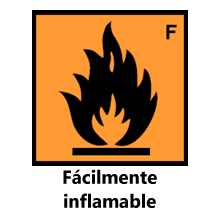
\includegraphics[width=3cm]{inflamable}
	\caption{Simbolo de sustancia fácilmente inflamable.}
	\end{figure}
\item Tóxicos: Las sustancias y preparados que, por inhalación; ingestión o penetración cutánea en pequeñas cantidades puedan provocar efectos agudos o crónicos e incluso la muerte.
\begin{figure}[H]
\centering

\includegraphics[width=4cm]{peligro}
\caption{Simbolo de sustancia tóxica.}
\end{figure} 
\item Nocivos: Las sustancias y preparados que, por inhalación, ingestión o penetración cutánea puedan provocar efectos agudos o crónicos e incluso la muerte.
\begin{figure}[H]
\centering
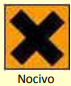
\includegraphics[width=2.5cm]{nocivo}
\caption{Simbolo de sustancia nociva.}
\end{figure} 
\item Corrosivos: Las sustancias y preparados que, en contacto con tejidos vivos puedan ejercer una acción destructiva de los mismos.
\begin{figure}[H]
\centering
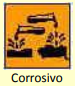
\includegraphics[width=2.5cm]{corrosivo}
\caption{Simbolo de sustancia corrosiva.}
\end{figure} 
\item Irritantes: Las sustancias y preparados no corrosivos que, en contacto breve, prolongado o repetido con la piel o las mucosas puedan provocar una reacción inflamatoria.
\begin{figure}[H]
\centering
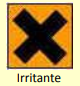
\includegraphics[width=2.5cm]{irritante}
\caption{Simbolo de sustancia irritante.}
\end{figure} 
\item Peligrosos para el medio ambiente: Las sustancias o preparados que presenten o puedan presentar un peligro inmediato o futuro para uno o más componentes del medio ambiente.
\begin{figure}[H]
\centering
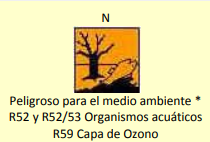
\includegraphics[width=6cm]{ambiente}
\caption{Simbolo de sustancia peligrosa para el ambiente.}
\end{figure} 
\end{enumerate}
\begin{figure}[H]
\centering
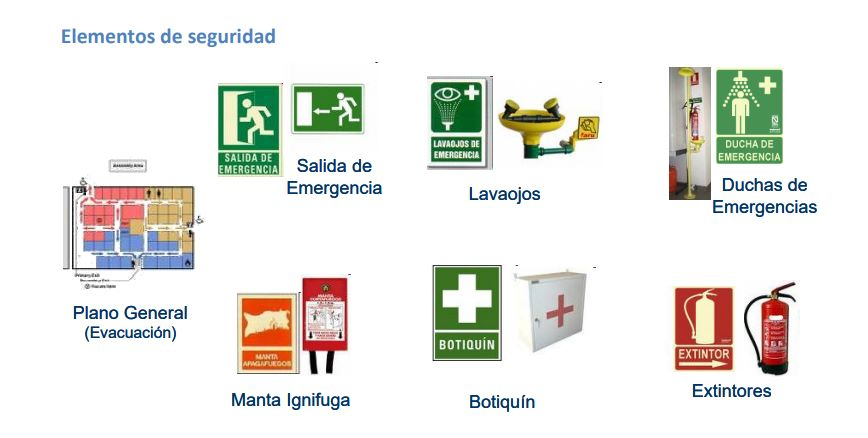
\includegraphics[width=8.5cm]{seguridad}
\caption{Elementos de seguridad.}
\end{figure} 

\subsection{Accidentes comunes en el laboratorio y cómo prevenirlos.}
Podemos prevenir estos accidentes siguiendo al pie de la letra recomendaciones expuestas en \cite{Seglab}:
\begin{itemize}
\item Realizar una lectura de la guía, para así estar enterados de cómo se va a realizar la práctica (para conocer el procedimiento). 
\item Asegurarnos de que disponemos de todo el material requerido. 
\item No manipular los químicos en exceso, siempre usar lo menos posible para evitar accidentes.
\item Llevar todos los elementos de bioseguridad necesarios, como bata, guantes, gafas, etc.
\item En caso de que algo llegase a suceder, es bueno contar siempre con un plan de actuación.
\end{itemize}

\subsection{Materiales del laboratorio examinados}

Véase cuadro \ref{tab:materiales}.

\subsection{Clasificacion del material de laboratorio}

Véase cuadro \ref{tab:clas-materiales}.

\section{Procedimiento experimental.}
En este experimento se midió el volumen de agua en un beaker utilizando una balanza analítica de presición, la cual es un método de medida gravimétrico según Skoog \cite{Skoog2004}. El procedimiento constó de los siguientes pasos:
\begin{enumerate}[1.]
\item Se midió la masa del beaker vacío utilizando una balanza analítica de precisión y se registró el valor en una tabla de datos.
\item Se agregaron 10 ml de agua al beaker y se midió la masa del beaker lleno de agua utilizando la misma balanza analítica de precisión. Se registró el valor en la tabla de datos.
\item Se calculó la diferencia entre la masa del beaker lleno de agua y la masa del beaker vacío para determinar la masa del agua contenida en el beaker. Este valor se registró en la tabla de datos.
\item Se utilizó la densidad del agua a temperatura ambiente para calcular el volumen del agua en el beaker. Este valor se obtuvo dividiendo la masa del agua por la densidad del agua y se registró en la tabla de datos.
\item Se repitió el procedimiento una vez por cada integrante del grupo para obtener un promedio del volumen de agua en el beaker.
\end{enumerate}

Después de realizado el procedimiento se obtubieron los siguientes datos:

\begin{table}[H]
\centering
\begin{tabular}{|p{1.8cm}|p{1.4cm}|p{1.6cm}|p{1.4cm}|}
\hline
 & \bfseries Peso del beaker & \bfseries Peso del beaker con agua & \bfseries Peso de agua \\
 & (g) & (g) & (g) \\
\hline
Joseph & 44.985 & 55.103 & 10.118 \\
\hline
Camilo & 44.986 & 55.037 & 10.051 \\
\hline
Juan Pablo & 44.960 & 55.046 & 10.086 \\
\hline
Jonathan & 44.970 & 55.070 & 10.100 \\
\hline
\end{tabular}
\caption{Medición de peso del agua con balanza de precisión.}
\label{tab:peso}
\end{table}

En base a estos datos y teniendo en cuenta que en \cite{atares} la densidad del agua es definida como 1 g/ml,  obtenemos:

\begin{table}[H]
\centering
\begin{tabular}{|p{2cm}|p{2cm}|p{2cm}|}
\hline
 & \bfseries Peso de agua & \bfseries Volumen de agua \\
 & (g) & (ml) \\
\hline
Joseph & 10.118 & 10.118 \\
\hline
Camilo & 10.051 & 10.051 \\
\hline
Juan Pablo & 10.086 & 10.086 \\
\hline
Jonathan & 10.100 & 10.100 \\
\hline
\end{tabular}
\caption{Calculo del volumen del agua.}
\label{tab:volumen}
\end{table}

\section{Analisis del error experimental}

La presición se refiere a la capacidad de repetir una medición y obtener resultados similares. Si las mediciones de todos son consistentes entre sí, es decir, si no hay mucha variación en los resultados, entonces se puede decir que la presición es alta.

La exactitud, por otro lado, se refiere a la proximidad de los resultados, entonces podemos decir que la exactitud es alta.

El error experimental es la diferencia entre el valor medido y el valor verdadero. Es normal que exista algún grado de error experimental en cualquier medición debido a diversas causas, como la presición del instrumento de medición, la habilidad del operador, las condiciones ambientales, etc. El objetivo es minimizar el error experimental para obtener mediciones precisas y exactas.

Algunos factores que pueden influir en el error experimental tratado son:

\begin{itemize}
\item La presición del instrumento de medición: si la balanza no es lo suficientemente precisa, las mediciones pueden variar significativamente entre los integrantes del grupo.
\item La habilidad del operador: si no se está familiarizado con la técnica de medición o no se realiza de manera consistente, las mediciones pueden variar.
\item Las condiciones ambientales: si hay cambios en la temperatura, la humedad o la presión atmosférica durante las mediciones, pueden afectar los resultados.
\item El volumen real de agua: si el volumen real de agua en el beaker no es exactamente de 10 ml, entonces todas las mediciones estarán desviadas del valor verdadero.
\end{itemize}

En conclusión, para obtener mediciones precisas y exactas del peso de 10 ml de agua usando un beaker y repitiendo entre los cuatro integrantes del grupo, se deben minimizar los errores experimentales y controlar los factores quepueden influir en ellos.

\printbibliography %Prints bibliography

% !TEX TS-program = xelatex
% !TEX encoding = UTF-8 Unicode
% !TEX author = Joseph Diaz

\begin{table*}[p]
%\centering
\begin{tabular}{|c|p{2.5cm}|p{10.5cm}|p{3cm}|}
\hline
& \bfseries Instrumento & \bfseries Uso & \bfseries Especificaciones \\
\hline
1 & Soporte universal & Sostenimiento & \\
\hline
2 & Pinzas para tubo de ensayo & Sujetar instrumentos mientras se calientan y/o se manipulan. & \\
\hline
3 & Decantador & Separación de líquidos inmiscibles. & 250 ml \\
\hline
4 & Pipeta & Medir la alícuota de un líquido con mucha presión. & 5 ml A . S \\
\hline
5 & Embudo & Se utiliza para el trasvasijado de productos químicos desde un recipiente a otro. & 60 mm \\
\hline
6 & Earlen-Meyer & Mide cantidades de líquidos. & 250 ml \\
\hline
7 & Tubos capilares & Mantienen controlada la presión con la que el flujo del refrigerante pasa entre el condensador y el evaporador y presentan resistencia al paso del refrigerante en estado líquido. & Micrometro 0-l6.5 C tm. \\
\hline
8 & Termometro & Mide la temperatura con un alto nivel de exactitud. & -10° hasta 200° \\
\hline
9 & Mezclador & Alcanzar procesos de mezcla, suspensión, dispersión, homogenización, transferencia de calor, etc. & \\
\hline
10 & Picnómetro & Mide con precisión la densidad de líquidos. & 25 ml \\
\hline
11 & Espatula & Romper, raspas, recoger y transferir productos químicos sólidos. & \\
\hline
12 & Mechero a gas & Calentar, esterilizar o proceder a la combustión de muestras o reactivos químicos. & \\
\hline
13 & Tubo de thiele & Contener y calentar un baño de aceite mineral o glicerina y se utiliza comúnmente en la determinación del punto de fusión de una sustancia. & \\
\hline
14 & Crisol & Calentar, fundir, quemar y calcinar sustancias. & \\
\hline
15 & Capsula de porcelana & Evaporar el exceso de solvente en una muestra. & \\
\hline
16 & Malla de asbesto &  Repartir la temperatura de manera uniforme cuando se calienta con un mechero. & \\
\hline
17 & Pinzas para crisol & Sostener y manipular capsulas de evaporación, crisoles y otros objetos. & \\
\hline
\end{tabular}
\caption{Matriz de los materiales suministrados.}
\label{tab:materiales}
\end{table*}

\begin{table*}[p]
\centering
\begin{tabular}{|c|c|c|}
\hline
\bfseries Material Volumétrico & \bfseries Material de Calentamiento & \bfseries Material de Sostenimiento \\
(Graduado o aforado) & & \\
\hline
 & & \\
\hline
 & & \\
\hline
 & & \\
\hline
 & & \\
\hline
\end{tabular}
\caption{Clasificación de los materiales observados.}
\label{tab:clas-materiales}
\end{table*}


\end{document}
